\chapter{Matematická optimalizace}\label{optimalizace}

Matematická optimalizace (jinak také matematické programování) je rozsáhlý obor zahrnující řadu disciplín, mezi které patří např. lineární a nelineární optimalizace, konvexní programování, celočíselné programování a jiné \cite{Bert}. Cílem této kapitoly je shrnout základní koncepty a techniky relevantní pro tuto práci. Nejprve představíme základní úlohu zkoumanou v rámci optimalizace, dále popíšeme některé z technik řešení úloh bez vazeb a s vazbami. Poté rozebereme optimalizaci úloh, v nichž obecně není známý předpis účelové funkce. Na závěr popíšeme celkový optimalizační rámec aplikovaný na optimalizaci úloh v této práci.

\section{Základní optimalizační úloha}

Buďte $ m, n, q \in \mathbb{N}$. Dále nechť jsou definovány spojité funkce $ f: \mathbf{D} \rightarrow \mathbb{R}$, $ \vec{g} : \mathbf{D} \rightarrow \mathbb{R}^m $, $ \vec{h} : \mathbf{D} \rightarrow \mathbb{R}^q $, kde $ \mathbf{D} = \mathrm{Dom} \, (f) \cap \mathrm{Dom} \, (g) \cap \mathrm{Dom} \, (h)$, tj. $ \mathbf{D} $ je průnik definičních oborů daných funkcí. Definujme množinu

\begin{equation}\label{eq:pripustna reseni}
\mathbf{X} = \big\{ \vec{x} \in \mathbf{D} \subseteq \mathbb{R}^n \ | \ \vec{g} (\vec{x}) \leq \vec{0} \wedge \vec{h} (\vec{x}) = \vec{0} \, \big\},
\end{equation}
kde nerovnost $ \vec{g} \leq \vec{0} $ a rovnost $ \vec{h} = \vec{0} $  jsou chápány po složkách. Obecně je pak cílem matematické optimalizace řešit úlohu

\begin{equation}\label{eq:zakladni uloha}
	\min_{\vec{x} \in \mathbf{X}} f(\vec{x}).
\end{equation}
Minimalizovanou funkci $ f $ nazýváme účelová funkce, množinu $ \mathbf{D} $ nazýváme definiční obor úlohy, $ \mathbf{X} $~se nazývá množina přípustných řešení \cite{Bert}. Upozorněme, že dále $ f $ bude značit pouze účelovou funkci, nikoliv distribuční funkce z kapitoly \ref{lbm}.

Při klasifikaci optimalizačních problémů hovoříme o tzv. vazbách. Ty jsou určeny definicí množiny~$ \mathbf{X} $, tj. rovnostními a nerovnostními podmínkami pro funkce $ \vec{g} $ a $ \vec{h} $, a tvarem množiny $ \mathbf{D} $. V případě podmínek definovaných $ \vec{g} (\vec{x}) \leq \vec{0} \wedge \vec{h} (\vec{x}) = \vec{0} $ hovoříme o explicitních vazbách, omezení definovaná definičním oborem úlohy $ \mathbf{D} $ nazýváme implicitní.

Prvek $ \vec{x}^{\star} \in  \mathbf{X} $ budeme nazývat optimálním řešením úlohy \eqref{eq:zakladni uloha} za předpokladu, že
\begin{equation}
	\vec{x}^{\star} = \operatorname*{argmin}_{\vec{x} \in \mathbf{X}} \, f(\vec{x}).
\end{equation}
Podotkněme, že optimální řešení nemusí být dáno jednoznačně a množinu všech optimálních řešení úlohy nazveme optimální množina. Je důležité zmínit, že hledání optimálního řešení lze ekvivalentně formulovat také jako hledání maxima z funkce $ -f $ přes stejnou množinu $ \mathbf{X}$, což umožnuje řešit problémy maximalizace pomocí stejných technik, které budou představeny dále \cite{Bert, non-linear-textbook}.

\section{Řešení úlohy bez vazeb}\label{unconstrained}

V této sekci rozebere řešení úlohy bez vazeb, tj. v úloze \eqref{eq:zakladni uloha} budeme předpokládat 
$ \mathbf{X} = \mathbb{R}^n $. Popíšeme pouze část metod, které lze pro řešení optimalizačních úloh bez vazeb použít. Konkrétně se zaměříme na tzv. kvazinewtonovské metody. Detailní popis metod pro řešení úloh bez vazeb lze najít např. v \cite{non-linear-textbook}.

Kvazinewtonovské metody jsou třídou gradientních metod. Mezi gradientní metody dále patří např.~metoda největšího spádu nebo metoda konjugovaných gradientů. Dále popsané algoritmy slouží k~nalezení~stacionárního bodu účelové funkce $ f $, tedy bodu $ \tilde{x} $ takového, že $ \nabla f(\tilde{x}) = 0 $. Za dodatečného předpokladu splnění vhodných podmínek lze pak usoudit, zda se jedná o hledaný globální extrém účelové funkce~\cite{Bert, non-linear-textbook}.

Kvazinewtonovské metody jsou iterativní a jejich hlavní myšlenkou je, že v každé iteraci používají k~určení směru spádu zlepšující se aproximace inverze Hessovy matice $ (\nabla ^2 f(\vec{x}))^{-1} $ založeném na algoritmu pro výpočet inverzní matice. K této aproximaci je v každé iteraci potřeba znalost gradientu účelové funkce. Výpočetní složitost kvazinewtonovských metod je obecně $ O(n^2) $, což poskytuje vylepšení ve srovnání s Newtonovou metodou, jejíž výpočetní složitost je $ O(n^3) $ \cite{non-linear-textbook}. Dále se zaměříme na dva konkrétní používané kvazinewtonovské algoritmy.

\subsection{Davidonův-Fletcherův-Powellův algoritmus}\label{DFP}
První představenou kvazinewtonovskou metodou je Davidonův-Fletcherův-Powellův (dále jen DFP) algoritmus \cite{Fletcher1963}. Dále budeme značit $ H_k $ aproximaci inverze Hessovy matice v $ k $-té iteraci, na začátku incializujeme $ H_0 = I $. Algoritmus DFP lze pak shrnout v následujících krocích:

\begin{enumerate}
	\item \textbf{Inicializace:} Volba $ \vec{x}_0 \in \mathbf{X}$ a následné vypočtení $ \vec{g}_0 = \nabla f (\vec{x}_0) $. Nastavení hodnot $ k=0 $ a $ H_0 = I $.
	\item \textbf{Cyklus} končící splněním podmínky ukončení, která je zadána uživatelem. Z důvodu konečné strojové přesnosti typicky požadujeme, aby vypočtená hodnota gradientu byla menší než požadovaný parametr $ \varepsilon > 0$.
	\begin{enumerate}
		\item \textbf{Vypočtení směru hledání} jako $ \vec{d}_k = -H_k \vec{g}_k $.
		\item \textbf{Jednorozměrná minimalizace}, při které najdeme $ \alpha_k = \operatorname*{argmin}_{\alpha \geq 0} f (\vec{x}_k + \alpha \vec{d}_k)$.
		\item \textbf{Vypočtení a nastavení hodnot:}
		\begin{subequations}
			\begin{eqnarray}
			\vec{x}_{k+1} &=& \vec{x}_k + \alpha_k \vec{d}_k,\\[3pt]
			\vec{g}_{k+1} &=& \nabla f({\vec{x}_{k+1}}).
			\end{eqnarray}
		\end{subequations}
		\item \textbf{Aproximace inverze Hessovy matice:} 
		\begin{subequations}
			\begin{eqnarray}
			\vec{p}_{k} &=& \vec{x}_{k+1} - \vec{x}_{k},\\[3pt]
			\vec{q}_{k} &=& \vec{g}_{k+1} - \vec{g}_{k},\\[3pt]\label{eq:hessian}
			H_{k+1} &=& H_k - \frac{1}{\vec{q}^T_k H_k \vec{q}^{}_k} (H_k \vec{q}^{}_k)(H_k \vec{q}^{}_k)^T + \frac{1}{\vec{p}^T_k \vec{q}^{}_k} (\vec{p}^{}_k \vec{p}^{T}_k).
			\end{eqnarray}
		\end{subequations}
		\item \textbf{Nastavení} $ k = k + 1 $.
	\end{enumerate}
	\item \textbf{Konec algoritmu.}
\end{enumerate}
Posloupnost vektorů $ \vec{x}_k $ v algoritmu konverguje k řešení úlohy. Jedním z teoretických výsledků týkajích se DFP algoritmu je fakt, že pro $ f $ konvexní konverguje ke stacionárnímu bodu pro libovolnou volbu počátečního vektoru $ \vec{x}_0 $ \cite{non-linear-textbook}.

\subsection{Broydenův-Fletcherův-Goldfarbův-Shannoův algoritmus}\label{BFGS}
Druhou kvazinewtonovskou metodou, kterou popíšeme, je Broydenův-Fletcherův-Goldfarbův-Shannoův (dále jen BFGS) algoritmus \cite{broyden1970}. BFGS algoritmus je modifikací DFP algoritmu, s kterým sdílí všechny jeho kroky, jedinou jeho odlišností je využití jiné aproximace inverze Hessovy matice. BFGS algoritmus nahrazuje rovnici \eqref{eq:hessian} vztahem
\begin{equation}
	H_{k+1} = H_k - \frac{1}{\vec{p}^{T}_{k} \vec{q}^{}_k} \left[ \vec{p}^{}_{k} (H_k \vec{q}^{}_k)^T + (H_k \vec{q}^{}_k) \vec{p}^T_k - \left( 1 + \frac{\vec{q}^T_k H_k \vec{q}^{}_k}{\vec{p}^T_k \vec{q}^{}_k} \right) (\vec{p}^{}_k \vec{p}^{T}_k) \right].
\end{equation}
Z hlediska konvergence se dá BFGS algoritmus považovat za lepší než DFP. Za zmínění stojí modifikace BFGS algoritmu jménem L-BFGS (nebo LM-BFGS, z anglického \textit{limited-memory BFGS}), která pracuje pouze s omezeným množstvím počítačové paměti, a proto je její využití vhodné pro úlohy s vyšší dimenzí~\cite{Byrd1995}.

\section{Řešení úlohy s vazbami}\label{constrained}
Budeme nyní uvažovat úlohu \ref{eq:zakladni uloha} z úvodu kapitoly, kde množina přípustných řešení má tvar \ref{eq:pripustna reseni}. V~této sekci popíšeme, jak tuto úlohu řešit převedením na posloupnost optimalizačních úloh bez vazeb, jejichž řešení bylo diskutováno v sekci \ref{unconstrained}. Opět existuje více způsobů, jak úlohy s vazbami řešit, zde však popíšeme pouze řešení pomocí penalizačních a bariérových metod.

\subsection{Penalizační metody}\label{penalty method}
Jak již bylo řečeno, penalizační metody převádí řešení omezených úloh na úlohy bez omezení. Základním principem penalizačních metod je zohlednění podmínek vymezujících množinu přípustných řešení tak, že k účelové funkci přidáme penalizační člen, který reflektuje míru překročení daných podmínek \cite{Bert}. Jako penalizační funkci budeme označovat spojitou skalární funkci na $ \mathbb{R}^n $ splňující

\begin{align}
\begin{split}
p(\vec{x}) &=0, \ \ \forall \vec{x} \in \mathbf{X},\\[6pt]
p(\vec{x}) &>0, \ \ \text { jinak. }
\end{split}
\end{align}
Typickou volbou penalizační funkce je např.
\begin{equation}\label{eq:penalty function}
p (\vec{x}) = \sum_{j=1}^{m} \left( \, \max  \left\{ \,  g_j (\vec{x}), 0 \,  \right\} \, \right)^2 + \sum_{j=1}^{q} h_j (\vec{x})^2.
\end{equation}


Pomocí penalizační funkce $ p $ dále sestrojíme modifikovanou účelovou funkci 
\begin{equation}\label{eq:cost function with penalty}
	\phi (\vec{x}, r) = f (\vec{x}) + r p(\vec{x}),
\end{equation}
kde $ r > 0 $ nazýváme penalizační parametr \cite{Bert}. Z definice penalizační funkce můžeme vidět, že hodnoty modifikované účelové funkce $ \phi (\vec{x}, r)$ jsou různé od původní funkce $ f $ pouze pro taková $ \vec{x} $, kdy je porušena zadaná zohledněná podmínka.

Pro řešení úlohy s vazbami budeme v každé iteraci konstruovat nový člen ostře rostoucí posloupnosti penalizačních parametrů $ r_1, r_2, \dots$, pro který budeme řešit optimalizační úlohu bez vazeb pro modifikovanou funkci $ \phi (\vec{x}, r_k)$. Optimální řešení $ \vec{x}_k $ této úlohy bez vazeb (nalezené např. technikami popsanými v sekci \ref{unconstrained}) využijeme jako počáteční bod pro další iteraci. Toto opakujeme dokud není splněna podmínka $ r_k p(\vec{x}_k) < \varepsilon$ pro zvolené $  \varepsilon > 0$, při splnění této podmínky lze $ \vec{x}_k $ považovat za postačující aproximaci řešené úlohy s vazbami. Podotkněme, že penalizační metody umožňují hledat optimální řešení během jednotlivých iterací mimo množinu přípustných řešení \cite{non-linear-textbook}, proto jsou řazeny mezi tzv. metody vnějšího bodu. Důležitým předpokladem penalizačních metod je, aby definiční obor úlohy splňoval $ \mathbf{D} = \mathbb{R}^n $.

Konstrukce posloupnosti penalizačních parametrů a princip penalizační metody je znázorněn na obr.~\ref{fig:penalty} na triviálním příkladu minimalizace funkce $ f(x) = 0,5x $ s podmínkou $ g(x) = 4 - x \leq 0 $. Modifikovaná účelová funkce má v tomto případě tvar 
\begin{equation}
	 \phi (x, r) = 0,5x + r \left(\max  \left\{ \,  4-x, 0 \right\}\right)^2.
\end{equation}

\begin{figure}[H]
	\centering
	\includegraphics[width=1.0\textwidth]{Images/penalty.pdf}
	\vspace{0.25cm}
	\caption{Ilustrace penalizační metody použité pro minimalizaci funkce $ f(x) = 0,5x $ s podmínkou $ g(x) = 4 - x \leq 0 $. Barevně jsou odlišeny různé tvary modifikované účelové funkce $\phi (x, r)  $ v závislosti na hodnotě penalizačního parametru $ r $. Podmínka vymezující množinu přípustných řešení je vyznačena šedě čárkovaně. Množina přípustných řešení se nachází v polorovině napravo od této šedé čárkované osy.}
	\label{fig:penalty}
\end{figure}

\subsection{Bariérová metoda}\label{barrier method}
Bariérová metoda využívá podobného principu jako penalizační metody, jejím hlavním rozdílem však je, že při iterativním hledání optimálního řešení úlohy s vazbami je garantováno, že odhady řešení vždy budou prvky vnitřku přípustné množiny, který má tvar
\begin{equation}
\mathbf{X}^{\mathrm{o}} = \big\{ \vec{x} \in \mathbf{D} \subseteq \mathbb{R}^n \ | \ \vec{g} (\vec{x}) < \vec{0} \, \big\}.
\end{equation}
Metody splňující tuto podmínku se obecně nazývají metody vnitřního bodu \cite{non-linear-textbook}.

Opět zohledníme podmínky vymezující množinu přípustných řešení tak, že k účelové funkci přidáme nový člen, který reflektuje míru jejich překročení. Jako bariérovou funkci $ B $ budeme chápat spojitou skalární funkci na $ \mathbf{X}^{\mathrm{o}} $ splňující podmínku
\begin{equation}
	(\exists j \in \{1,2,\dots,m\})(\lim\limits_{\substack{\vec{x} \to \vec{y} \\ \mathbf{X}^{\mathrm{o}}}} g_j (\vec{x}) = 0) \Rightarrow \lim\limits_{\substack{\vec{x} \to \vec{y} \\ \mathbf{X}^{\mathrm{o}}}} B (\vec{x}) = + \infty.
\end{equation}
Typickou volbou bariérové funkce je např. logaritmická bariérová funkce
\begin{equation}\label{eq:log barrier function}
B (\vec{x}) = -\sum_{j=1}^{m} \ln \left( \, - g_j (\vec{x}) \right),
\end{equation}
nebo dále např. reciproká bariérová funkce
\begin{equation}\label{eq:reciprocal barrier function}
B (\vec{x}) = -\sum_{j=1}^{m} \frac{1}{g_j (\vec{x})}.
\end{equation}
Pomocí barierové funkce $ B $, podobně jako u penalizačních metod, sestrojíme modifikovanou účelovou funkci 
\begin{equation}\label{eq:cost function with barrier}
\phi (\vec{x}, r) = f (\vec{x}) + r B(\vec{x}),
\end{equation}
kde $ r > 0 $ je volený parametr \cite{non-linear-textbook}.

Pro řešení úlohy s vazbami pomocí bariérové metody budeme v každé iteraci konstruovat nový člen kladné ostře klesající posloupnosti parametrů $ r_1, r_2, \dots$, pro který budeme řešit optimalizační úlohu bez vazeb pro modifikovanou funkci $ \phi (\vec{x}, r_k)$. Vektor $ \vec{x}_k  = \operatorname*{argmin}_{\vec{x} \in \mathbf{X}^\mathrm{o}} (f (\vec{x}) + r_k B(\vec{x}))$ určený optimalizací úlohy bez vazeb využijeme jako počáteční bod pro další iteraci. Toto opakujeme dokud není splněna podmínka $ r_k < \varepsilon$ pro zvolené $  \varepsilon > 0$, při splnění této podmínky $ \vec{x}_k $ považujeme za postačující aproximaci řešené úlohy s vazbami \cite{non-linear-textbook}.

Dále zmíníme volbu bariérové funkce $ B_{\infty} $ využívané k definici tzv. extrémní bariérové funkce (anglicky \textit{extreme barrier function}), jak se nazývá modifikovaná účelová funkce při této volbě \cite{BBO-textbook}. Tato bariérová funkce kopíruje asymptotické chování výše zmíněných bariérových funkcí a má tvar
\begin{align}
\begin{split}
B_{\infty}(\vec{x}) &=0, \ \ \forall \vec{x} \in \mathbf{X},\\[6pt]
B_{\infty}(\vec{x}) &=+\infty, \ \ \text { jinak. }
\end{split}
\end{align}
Modifikovaná účelová funkce (extrémní bariérová funkce) má pak tvar
\begin{align}\label{eq:extreme barrier}
\begin{split}
f_{\infty}(\vec{x}) &=f(\vec{x}) , \ \ \forall \vec{x} \in \mathbf{X},\\[6pt]
f_{\infty}(\vec{x}) &=+\infty, \ \ \text { jinak. }
\end{split}
\end{align}

Konstrukce posloupnosti parametrů $ (r_k)_{k \in \mathbb{N}} $ a princip bariérové metody je znázorněn na obr.~\ref{fig:barrier} opět na příkladu minimalizace funkce $ f(x) = 0,5x $ s podmínkou $ g(x) = 4 - x \leq 0 $ a volbou reciproké bariérové funkce. Modifikovaná účelová funkce má tvar 
\begin{equation}
\phi (x, r) = 0,5x - \frac{r}{4-x}.
\end{equation}

\begin{figure}[H]
	\centering
	\includegraphics[width=1.0\textwidth]{Images/barrier.pdf}
	\caption{Ilustrace bariérové metody použité pro minimalizaci funkce $ f(x) = 0,5x $ s podmínkou $ g(x) = 4 - x \leq 0 $. Barevně jsou odlišeny různé tvary modifikované účelové funkce $\phi (x, r)  $ v závislosti na hodnotě penalizačního parametru $ r $. Podmínka vymezující množinu přípustných řešení je vyznačena šedě čárkovaně. Množina přípustných řešení se nachází v polorovině napravo od této šedé čárkované osy.}
	\label{fig:barrier}
\end{figure}

\section{Black-box optimalizace}\label{black-box}
V praxi je běžné setkat se s případy, kdy je nutné v rámci řešení úlohy optimalizovat účelovou funkci~$ f $, jejíž analytický předpis stejně jako předpis pro výpočet derivace není známý. Tento problém je typický např. pro výsledky numerických simulací, kdy účelovou funkci dokážeme pouze vyčíslit v konkrétním bodě a získat tak požadovanou funkční hodnotu. Často pak v praxi také samotné vyčíslení funkce v bodě může představovat problém a může být např. velmi časově nebo výpočetně náročné. Zjevně pro řešení problémů tohoto charakteru není vhodné použít výše zmíněné standardní optimalizační algoritmy.

Řešením úloh, v kterých je účelová funkce (popř. i zadané vazby) dána pomocí tzv. black-boxu\footnote{Jako black-box se v programování označuje systém, jehož vnitřní mechanismy nejsou uživateli známy. To znamená, že uživateli je přístupný obecně pouze vstup a výstup daného systému \cite{BBO-textbook}.}, se zabývá disciplína jménem black-box optimalizace (dále jen BBO). V rámci BBO typicky není předpokládáno, že by účelová funkce byla spojitá nebo diferencovatelná \cite{BBO-textbook, derivative-free-review, two-decades}.

Podotkněme, že v literatuře se často black-box optimalizace zaměňuje s bezgradientní optimalizací (anglicky \textit{derivative-free optimization}, dále jen DFO), která zahrnuje metody a techniky pro účelové funkce, jejichž derivace není známa či je obtížné ji vypočítat \cite{BBO-textbook, derivative-free-review, Kramer2011}. Tyto dvě disciplíny sdílí řadu společných vlastností, liší se však zejména v tom, že v rámci DFO může být předpis pro výpočet derivace účelové funkce známý. Dále BBO v sobě zarhnuje i heuristické metody, zatímco DFO se zaměřuje zejména na metody, které mohou být spolehlivě matematicky analyzovány z hlediska konvergence a stanovení zastavovací podmínky, což pro metody BBO mnohdy není možné \cite{BBO-textbook}. Proto ačkoliv, jak bylo zmíněno, se pojmy BBO a DFO často zaměňují, v rámci této práce je budeme chápat jako dvě rozdílné disciplíny \cite{BBO-textbook}.

Dále podotkněme, že v literatuře lze najít různé klasifikace metod v rámci BBO. V rámci této práce se budeme držet klasifikace uvedené v \cite{BBO-textbook} a budeme tedy odlišovat heuristické metody, metody přímého vyhledávání a metody založené na využití náhradního modelu. Každou z těchto tříd v této sekci krátce popíšeme.

\subsection{Heuristické metody}\label{heuristic}
Mezi heuristické optimalizační metody patří mimo jiné třída genetických algoritmů, která je blíže popsána v \cite{BBO-textbook} společně s dalšími různými heuristickými metodami. V této sekci popíšeme jinou používanou heuristickou metodu, a to Nelderovu-Meadovu metodu (v textu dále někdy označována zkratkou NM), také někdy označovanou jako simplexová\footnote{Simplexem v $ \mathbb{R}^n $ nazýváme omezený konvexní polytop (zobecnění mnohostěnu v libovolné dimenzi) s neprázdným vnitřkem a právě $ n+1 $ vrcholy \cite{BBO-textbook}.} metoda\footnote{Jako simplexová metoda je v rámci optimalizace častěji označovaný algoritmus sloužící pro nalezení optimálního řešení lineárního programování. Autorem tohoto algoritmu je George Dantzig \cite{Dantzig1990}.}\cite{Nelder1965}.

Nelderova-Meadova metoda, využívá k optimalizaci iterativní konstrukci simplexů. Na jejím začátku je zvolen počáteční simplex a účelová funkce je vyčíslena v každém z vrcholů tohoto simplexu. V každé další iteraci algoritmu je daný simplex transformován tak, aby lépe odpovídal pozici hledaného stacionárního bodu účelové funkce. Transformace simplexu probíhá v každé iteraci manipulací jeho bodů pomocí operací prodloužení, zrcadlení, zmenšení a kontrakce (vnitřní a vnější), které jsou schematicky zobrazeny na obr.~\ref{fig:NM operations}. Operace, které se provedou během iterace, jsou určeny porovnáním hodnot funkce ve vrcholech simplexu. Nově vzniklý simplex sdílí se simplexem z předchozí iterace buď právě jeden, nebo právě $ n $ vrcholů. Algoritmus pokračuje v iterativní transformaci simplexu, dokud není splněna podmínka ukončení, která musí být blíže specifikována uživatelem \cite{BBO-textbook}. Detaily ohledně Nelderovy-Meadovy metody zahrnující popis algoritmu a volby podmínky ukončení jsou rozebrány např. v \cite{BBO-textbook, derivative-free-review, Nelder1965}.

\begin{figure}[H]
	\vspace{5mm}
	\centering
	\includegraphics[width=0.76\textwidth]{Images/neldermead.pdf}
	\vspace{2mm}
	\caption{Schéma operací používaných k transformaci simplexů v rámci Nelderovy-Meadovy metody. Vrcholy vzniklé aplikací dané operace jsou vyznačeny červeně. Pro názornost jsou operace vyobrazeny v $ \mathbb{R}^2 $.}
	\vspace{2mm}
	\label{fig:NM operations}
\end{figure}


Heuristický charakter Nelderovy-Meadovy metody vyplývá z toho, že její princip je postaven na do jisté míry náhodném prohledávání prostoru pomocí předem definovaných pravidel. Několik iterací prohledávání prostoru pomocí simplexů je pro konkrétní volbu počátečního simplexu a konkrétní funkci znázorněno na obr. \ref{fig:NM}. Je dokázána konvergence této metody, není však zaručeno, že metoda vždy nutně konverguje ke stacionárnímu bodu \cite{BBO-textbook}. Podotkněme, že Nelderova-Meadova metoda je primárně odvozena pro optimalizaci úloh bez vazeb, lze však použít techniky popsané v sekci \ref{unconstrained} a použít ji pro optimalizaci úloh s vazbami.

%\begin{figure}[H]
%	\centering
%	\includegraphics[width=0.99\textwidth]{Images/nelder.png}
%	\vspace{2mm}
%	\caption{Několik iterací Nelderovy-Meadovy metody pro konkrétní volbu počátečního simplexu při minimalizaci funkce $ x^2 - 4x + y^2 - y - xy + 7 $ s minimem v bodě (3,2) znázorněným červeným křížkem.}
%	\vspace{2mm}
%	\label{fig:NM}
%\end{figure}

\begin{figure}[H]
	\vspace{-2mm}
	\begin{subfigure}[b]{0.32\textwidth}
		\centering
%		trim={<left> <lower> <right> <upper>}
		\includegraphics[width=0.96\textwidth, trim={0 0 0 0}, clip]{Images/nelder1.pdf}
	\end{subfigure}
	\begin{subfigure}[b]{0.32\textwidth}
		\centering
		\includegraphics[width=0.96\textwidth, trim={0 0 0 0}]{Images/nelder2.pdf}
	\end{subfigure}
	\vspace{1mm}
	\begin{subfigure}[b]{0.32\textwidth}
		\centering
		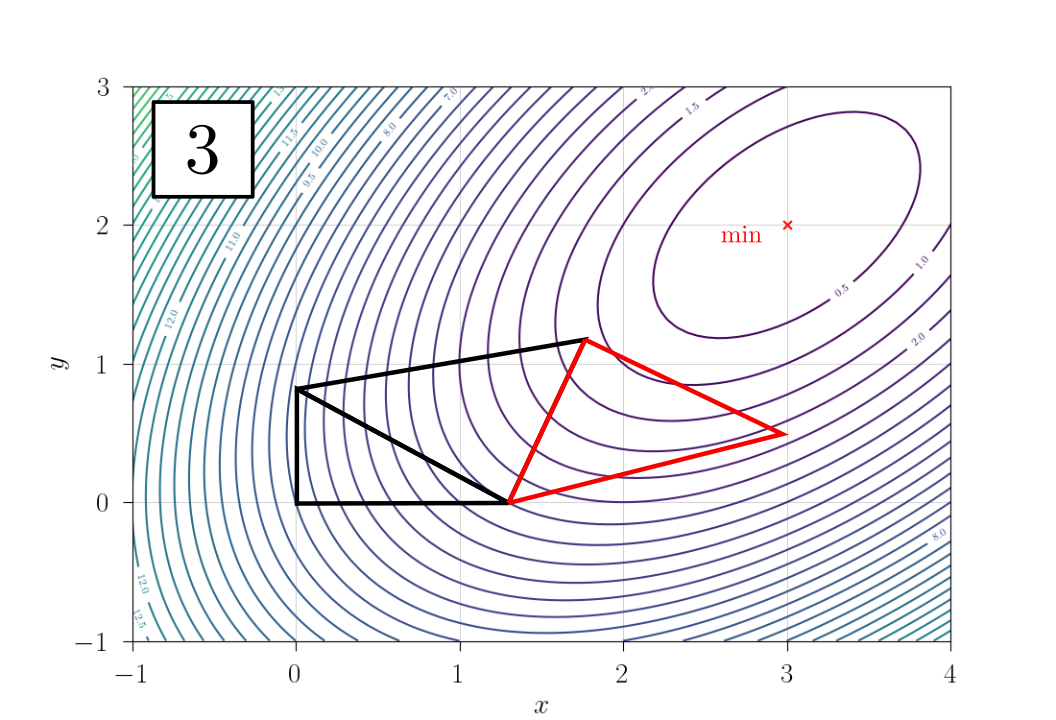
\includegraphics[width=0.96\textwidth, trim={0 0 0 0}]{Images/nelder3.pdf}
	\end{subfigure}
	\vspace{1mm}
	\begin{subfigure}[b]{0.32\textwidth}
		\centering
		\includegraphics[width=0.96\textwidth, trim={0 0 0 0}]{Images/nelder4.pdf}
	\end{subfigure}
	\begin{subfigure}[b]{0.32\textwidth}
		\centering
		\includegraphics[width=0.96\textwidth, trim={0 0 0 0}]{Images/nelder5.pdf}
	\end{subfigure}
	\begin{subfigure}[b]{0.32\textwidth}
		\centering
		\includegraphics[width=0.96\textwidth, trim={0 0 0 0}]{Images/nelder6.pdf}
	\end{subfigure}
	\centering
	\begin{subfigure}[b]{0.32\textwidth}
		\centering
		\includegraphics[width=0.96\textwidth, trim={0 0 0 0}]{Images/nelder7.pdf}
	\end{subfigure}
	\begin{subfigure}[b]{0.32\textwidth}
		\centering
		\includegraphics[width=0.96\textwidth, trim={0 0 0 0}]{Images/nelder8.pdf}
	\end{subfigure}
	\begin{subfigure}[b]{0.32\textwidth}
		\centering
		\includegraphics[width=0.96\textwidth, trim={0 0 0 0}]{Images/nelder9.pdf}
	\end{subfigure}
	\begin{center}
		\begin{subfigure}[b]{0.66\textwidth}
			\centering
			\includegraphics[width=0.985\textwidth, trim={0 6mm 0 9mm}]{Images/nelder.png}
		\end{subfigure}
	\end{center}

	\caption{Několik iterací Nelderovy-Meadovy metody pro konkrétní volbu počátečního simplexu při minimalizaci funkce $ x^2 - 4x + y^2 - y - xy + 7 $ s minimem v bodě (3,2) znázorněným červeným křížkem.}
	\label{fig:NM}
\end{figure}


\subsection{Metody přímého vyhledávání}\label{direct-search}
Z metod přímého vyhledávání popíšeme \textit{generalised pattern search} (dále jen GPS) metodu \cite{Audet2002} a~krátce zmíníme také \textit{mesh adaptive direct search} (dále jen MADS) metodu \cite{Audet2006}.

Pro popis algoritmu GPS je nutné definovat síť, pomocí níž je pak popsáno prohledávání prostoru v~rámci GPS. Buďte $ \mathbf{G} \in \mathbb{R}^{n \times n} $ a $ \mathbf{Z} \in \mathbb{Z}^{n \times p} $. Nechť  každý vektor z $ \mathbb{R}^{n} $ lze vyjádřit jako lineární kombinaci sloupců matice $ \mathbf{Z} $ (vnímaných jako vektory) tak, že všechny koeficienty v této lineární kombinaci jsou nezáporné. Dále označme $ \mathbf{S} = \mathbf{G} \mathbf{Z}$. Síť $ \mathbf{M} $ generovanou pomocí $ \mathbf{S} $ středovanou v bodě $ \vec{x} $ definujeme jako
\begin{equation}
	\mathbf{M} = \left\{ \vec{x} + \delta \, \mathbf{S} y \, | \, y \in \mathbb{N}^p \right\},
\end{equation}
kde $ \delta $ je parametr, jenž budeme nazývat síťový krok \cite{BBO-textbook, Audet2002}. V jednotlivých iteracích algoritmu GPS se obecně mění tvar sítě, jelikož je vždy středována v bodě představující nejlepší odhad v dané iteraci, dále se také mění velikost síťového kroku. Označíme-li $ \vec{x}_k $, resp. $ \delta_k $ jako odhad řešení, resp. síťový krok  v $ k $-té iteraci, můžeme definovat síť v $ k $-té iteraci označenou $ \mathbf{M} _k$, tj.
\begin{equation}
\mathbf{M} _k = \left\{ \vec{x}_k + \delta_k \, \mathbf{S} y \, | \, y \in \mathbb{N}^p \right\}.
\end{equation}
Poznamenejme, že sloupce výše definované matice $ \mathbf{S} $ lze chápat jako možné směry, kterými lze v rámci GPS prohledávat prostor hodnot optimalizačních parametrů \cite{BBO-textbook, Audet2002}.

Po inicializaci nutných počátečních parametrů je samotný algoritmus GPS v každé iteraci rozdělen do dvou hlavních kroků. Prvním krokem je tzv. hledání (anglicky \textit{search step}). Během kroku hledání je pomocí strategie blíže specifikované uživatelem vybrána konečná množina kandidátních síťových bodů, v nichž je vyčíslena účelová fukce. Pokud žádná z vypočtených hodnot nepředstavuje zlepšení oproti hodnotě $ f(\vec{x}_k) $, nastává krok průzkumu (anglicky \textit{poll step}). V kroku průzkumu je účelová funkce vyčíslena ve všech sousedních síťových bodech bodu $ \vec{x}_k $. V případě, že ani pak žádná z vypočtených hodnot nepředstavuje zlepšení oproti hodnotě $ f(\vec{x}_k) $, nastavíme $ \vec{x}_{k+1} = \vec{x}_k $ a snížíme hodnotu síťového kroku, tedy  $ \delta_{k+1} < \delta_k $. Pokud však v kroku hledání nebo v kroku průzkumu najdeme takový bod, pro který dojde k vylepšení odhadu řešení, označíme tento bod jako $ \vec{x}_{k+1} $ a zvýšíme hodnotu síťového kroku, tedy  $ \delta_{k+1} > \delta_k $ \cite{BBO-textbook, Audet2002}.

Výše popsané změny v každé iteraci vždy definují novou síť $ \mathbf{M} _k$, která se během algoritmu GPS obecně mění. Algoritmus je ukončen, když je splněno $ \delta_{k+1} < \varepsilon $ pro uživatelem specifikované $ \varepsilon > 0 $. Lze ukázat, že během GPS algoritmu konverguje krok sítě limitně k nule a za splnění vhodných předpokladů odhady řešení konvergují ke stacionárnímu bodu účelové funkce, detaily lze najít v \cite{BBO-textbook}. Podotkněme, že konvergence GPS je dokázána pro úlohy bez vazeb \cite{BBO-textbook}.

Dále krátce zmíníme metodu MADS, která představuje vylepšení metody GPS. Narozdíl od metody GPS, algoritmus MADS umožní během kroku průzkumu obecně zkoumat hodnoty účelové funkce ve směrech, které tvoří hustou podmnožinu v $ \mathbb{R}^{n} $ \cite{BBO-textbook, derivative-free-review}. Toto zobecnění vylepšuje konvergenci algoritmu a umožňuje dokázat konvergenci MADS i pro úlohy s vazbami, kdy je účelová funkce modifikována na extrémní bariérovou funkci \ref{eq:extreme barrier}. Detaily týkající se algoritmu a fungování metody MADS lze najít např.~v~\cite{BBO-textbook}.

\subsection{Optimalizace s využitím náhradního modelu}\label{model-based}
V případech, kdy je vyčíslení účelové funkce v konkrétním bodě časově nebo výpočetně  náročné, je užitečné během optimalizace v nějaké formě využít náhradu účelové funkce. Definujeme náhradní model (anglicky \textit{surrogate model}) zkoumané úlohy jako úlohu
\begin{equation}
	\min_{\vec{x} \in \mathbf{\tilde{X}}} \tilde{f}(\vec{x}),
\end{equation}
kde
\begin{equation}
\mathbf{\tilde{X}} = \big\{ \vec{x} \in \mathbf{D} \subseteq \mathbb{R}^n \ | \ \vec{\tilde{g}} (\vec{x}) \leq \vec{0} \wedge \vec{\tilde{h}} (\vec{x}) = \vec{0} \, \big\},
\end{equation}
přičemž funkce $ \tilde{f}, \vec{\tilde{g}}$ a $ \vec{\tilde{h}} $ mají podobný charakter, jako funkce $ f, \vec{g} $ a $ \vec{h}$ z původní úlohy. Charakter funkcí $ \tilde{f}, \vec{\tilde{g}}$ a $ \vec{\tilde{h}} $ je záměrně vymezen neurčitě - tento způsob definice odpovídá tomu, že po náhradním modelu nutně nepožadujeme, aby byl vhodným aproximativním modelem původní úlohy \cite{two-decades, BBO-textbook, Kramer2011}. Dobrý aproximativní model totiž nemusí být z hlediska optimalizace vhodnou náhradou, tato situace je znázorněna na obr. \ref{fig:surrogate}.

\begin{figure}[H]
	\centering
	\includegraphics[width=0.6\textwidth]{Images/surrogate.pdf}
	\caption{Ilustrace dvou náhradních modelů $ s_1 $ a $ s_2 $. Černě jsou vyznačeny hodnoty účelové funkce vykazující šum. Použití náhradního modelu $ s_1 $ představuje volbu lepší z hlediska aproximace funkce, pro optimalizaci však tato volba vhodná není, jelikož $ s_1 $ obsahuje mnoho nežádoucích stacionárních bodů, které původní účelová funkce nemá. Na druhou stranu náhradní model $ s_1$ vhodně neaproximuje účelovou funkci ve smyslu funkčních hodnot, z hlediska optimalizace jde však o lepší volbu, jelikož stacionární body $ s_2$ se nacházejí na téměř shodných pozicích, jako je tomu u optimalizované účelové funkce.}
	\label{fig:surrogate}
\end{figure}

Využití náhradního modelu v rámci optimalizace je většinou dílčí částí jiné obecné optimalizační metody. Náhradní modely lze např. použít v rámci metod GPS a MADS popsaných v sekci \ref{direct-search}, kdy při vyčíslování účelové funkce v kroku průzkumu nejdříve vyčíslíme v těch samých bodech náhradní funkci $ \tilde{f} $, tyto hodnoty pak seřadíme, a již seřazenou množinu bodů použijeme k vyčíslení původní funkce $ f $. To nám umožní potenciálně výrazně zkrátit čas, který je potřebný k provedení kroku průzkumu, jelikož seřazením bodů zvýšíme pravděpodobnost, že úspěšně najdeme lepší odhad řešení již pro jeden z prvních zkoumaných bodů \cite{BBO-textbook}. Náhradní modely lze použít i v rámci jiných metod a urychlit tak jejich průběh, detailně je jejich použití rozebráno např. v \cite{two-decades, BBO-textbook}.


\section{Popis optimalizačního rámce}\label{ramec}
Pro použití popsaných optimalizačních metod v rámci problematiky dynamiky tekutin a numerických simulací je potřeba vytvořit plně automatizovaný optimalizační rámec. Je vhodné navrhnout takový rámec, jehož jednotlivé části budou dostatečně modulární, tedy v případě potřeby může být pro vykonání specifického úkonu v rámci procesu optimalizace snadno použita jiná metoda. Celkový navržený rámec zahrnuje několik částí, které dále popíšeme:

\begin{enumerate}
	\item \textit{Optimalizace}: První část zahrnuje samotnou použitou optimalizační metodu, která řídí celý další proces. V této části je definována řešená úloha společně s případnými požadovanými vazbami. Jak již bylo zmíněno, je vhodné, aby tato část byla co nejvíce nezávislá na ostaních částech popisovaného optimalizačního rámce. To nám dovolí použít různé metody implementované v jiných programovacích jazycích bez narušení chodu celkového procesu.
	
	V této práci budeme pracovat s metodami L-BFGS (viz sekce \ref{BFGS}) a Nelderovou-Meadovou metodou (viz sekce \ref{heuristic}). Pro implementeci obou těchto metod použijeme volně dostupný balík \texttt{Optim.jl} \cite{Optim.jl} implementovaný v programovacím jazyce Julia. Pro zahrnutí vazeb použijeme v obou případech metodu transformující účelovou funkci na extrémní bariérovou funkci, která byla pro účely této práce implementována nad rámec použitého balíku. Pro výpočet gradientu v rámci metody L-BFGS použijeme automatickou diferenciaci, která je dostupná v rámci balíku \texttt{Optim.jl} a jejíž detaily jsou popsány v \cite{Optim.jl}. Metodu L-BFGS s toutou volbou výpočtu gradientu budeme dále značit L-BFGS(A).
	
	Dále v rámci optimalizačního rámce zařazujeme metodu přímého vyhledávání MADS (viz sekce \ref{direct-search}) implementovanou v programovacím jazyce C++ ve volně dostupné knihovně \texttt{NOMAD} \cite{nomad}. Pro zarhnutí vazeb rovněž použijeme extrémní bariérovou funkci, která je v případě knihovny \texttt{NOMAD} její součástí. Podotkněme, že v rámci této práce metoda MADS není využita.
	
	\item \textit{Generování geometrie}: Optimalizační parametry, jejichž hodnota se v každé iteraci optimalizace mění, jsou předány do generátoru geometrie. Pro generování geometrie, která je dále využita v numerické simulaci, byl použit balík \texttt{meshgenerator} implementovaný v jazyce Python. Zmíněný balík vznikl pro účely této práce a je blíže popsán v kapitole \ref{geometrie}.
	
	\item \textit{Numerická simulace}: Poslední částí optimalizačního rámce je řešič umožňující vyčíslení optimalizované účelové funkce. V rámci této práce se zabýváme pouze problémy týkajícími se dynamiky tekutin. Pro numerickou simulaci proudění byla použita metoda LBM, která je společně s implementačními poznámkami popsána v kapitole \ref{lbm}.
	
\end{enumerate}
Schématicky je propojení jednotlivých částí optimalizačního rámce zobrazeno na obr. \ref{fig:framework}.

\begin{figure}[H]
	\vspace{8mm}
	\centering
	\includegraphics[width=0.85\textwidth]{Images/framework.pdf}
	\vspace{7mm}
	\caption{Schématické znázornění navrženého optimalizačního rámce. Šipkami je znázorněno propojení jednotlivých částí, nad šipkou je pak zdůrazněno, co jednotlivé části předávají v procesu dále.}
	\label{fig:framework}
\end{figure}
